
In this section we describe the datasets and the methods we employed to answer the research questions posited in the earlier sections. 
\begin{figure*}[]
\begin{center}
%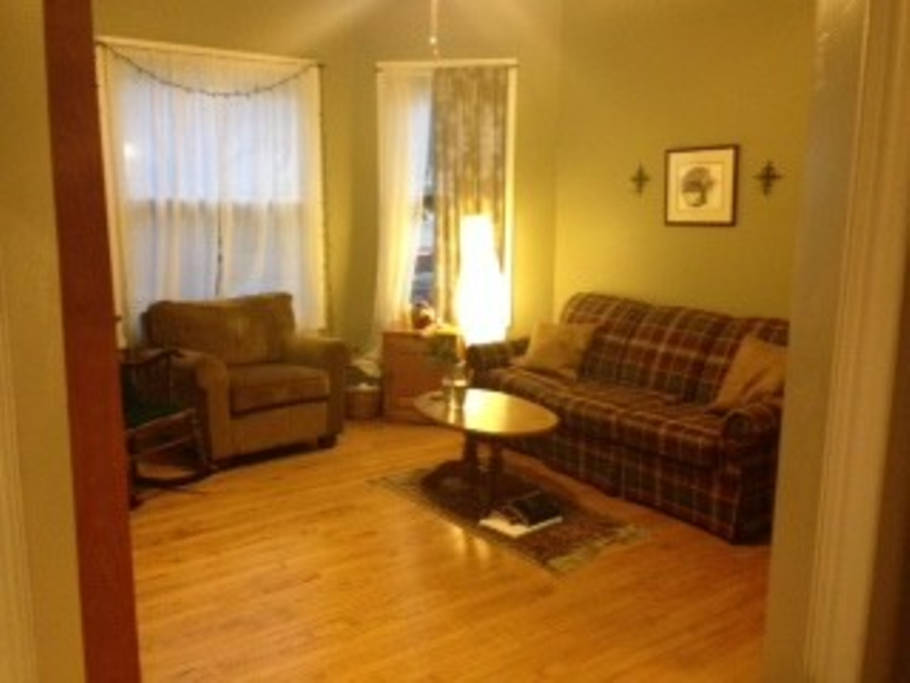
\includegraphics[width=0.5\columnwidth ]{pics/low/915372.jpg}
%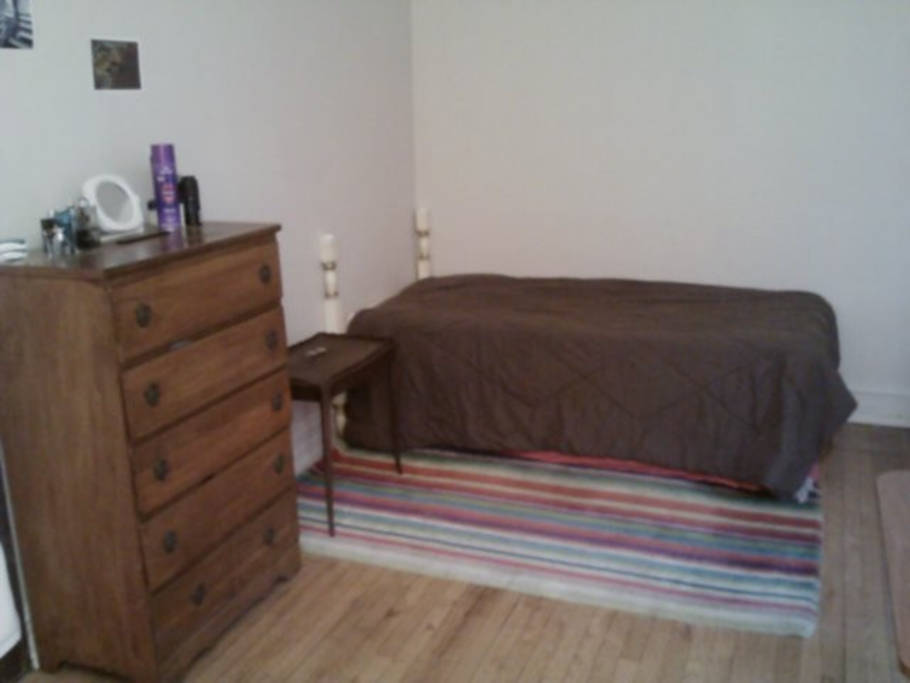
\includegraphics[width=0.5\columnwidth ]{pics/low/13892310.jpg}
%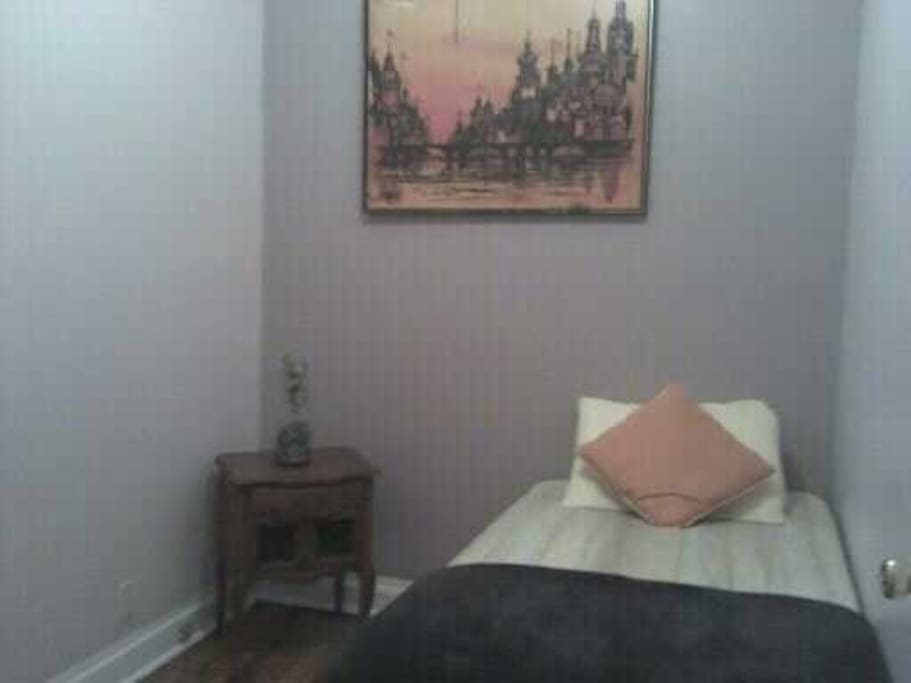
\includegraphics[width=0.5\columnwidth ]{pics/low/10227627.jpg}
%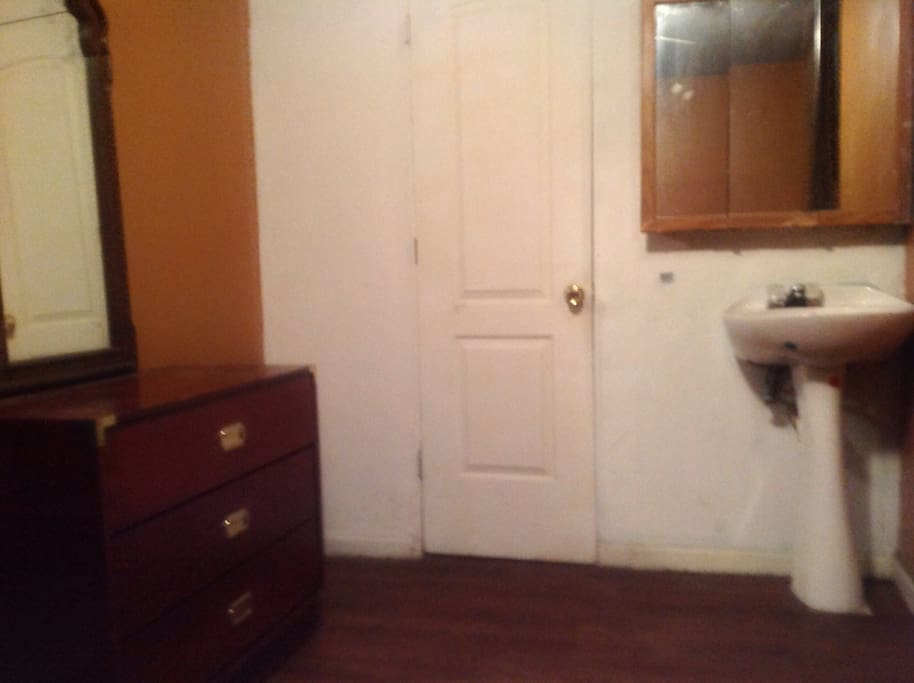
\includegraphics[width=0.5\columnwidth ]{pics/low/3751869.jpg}
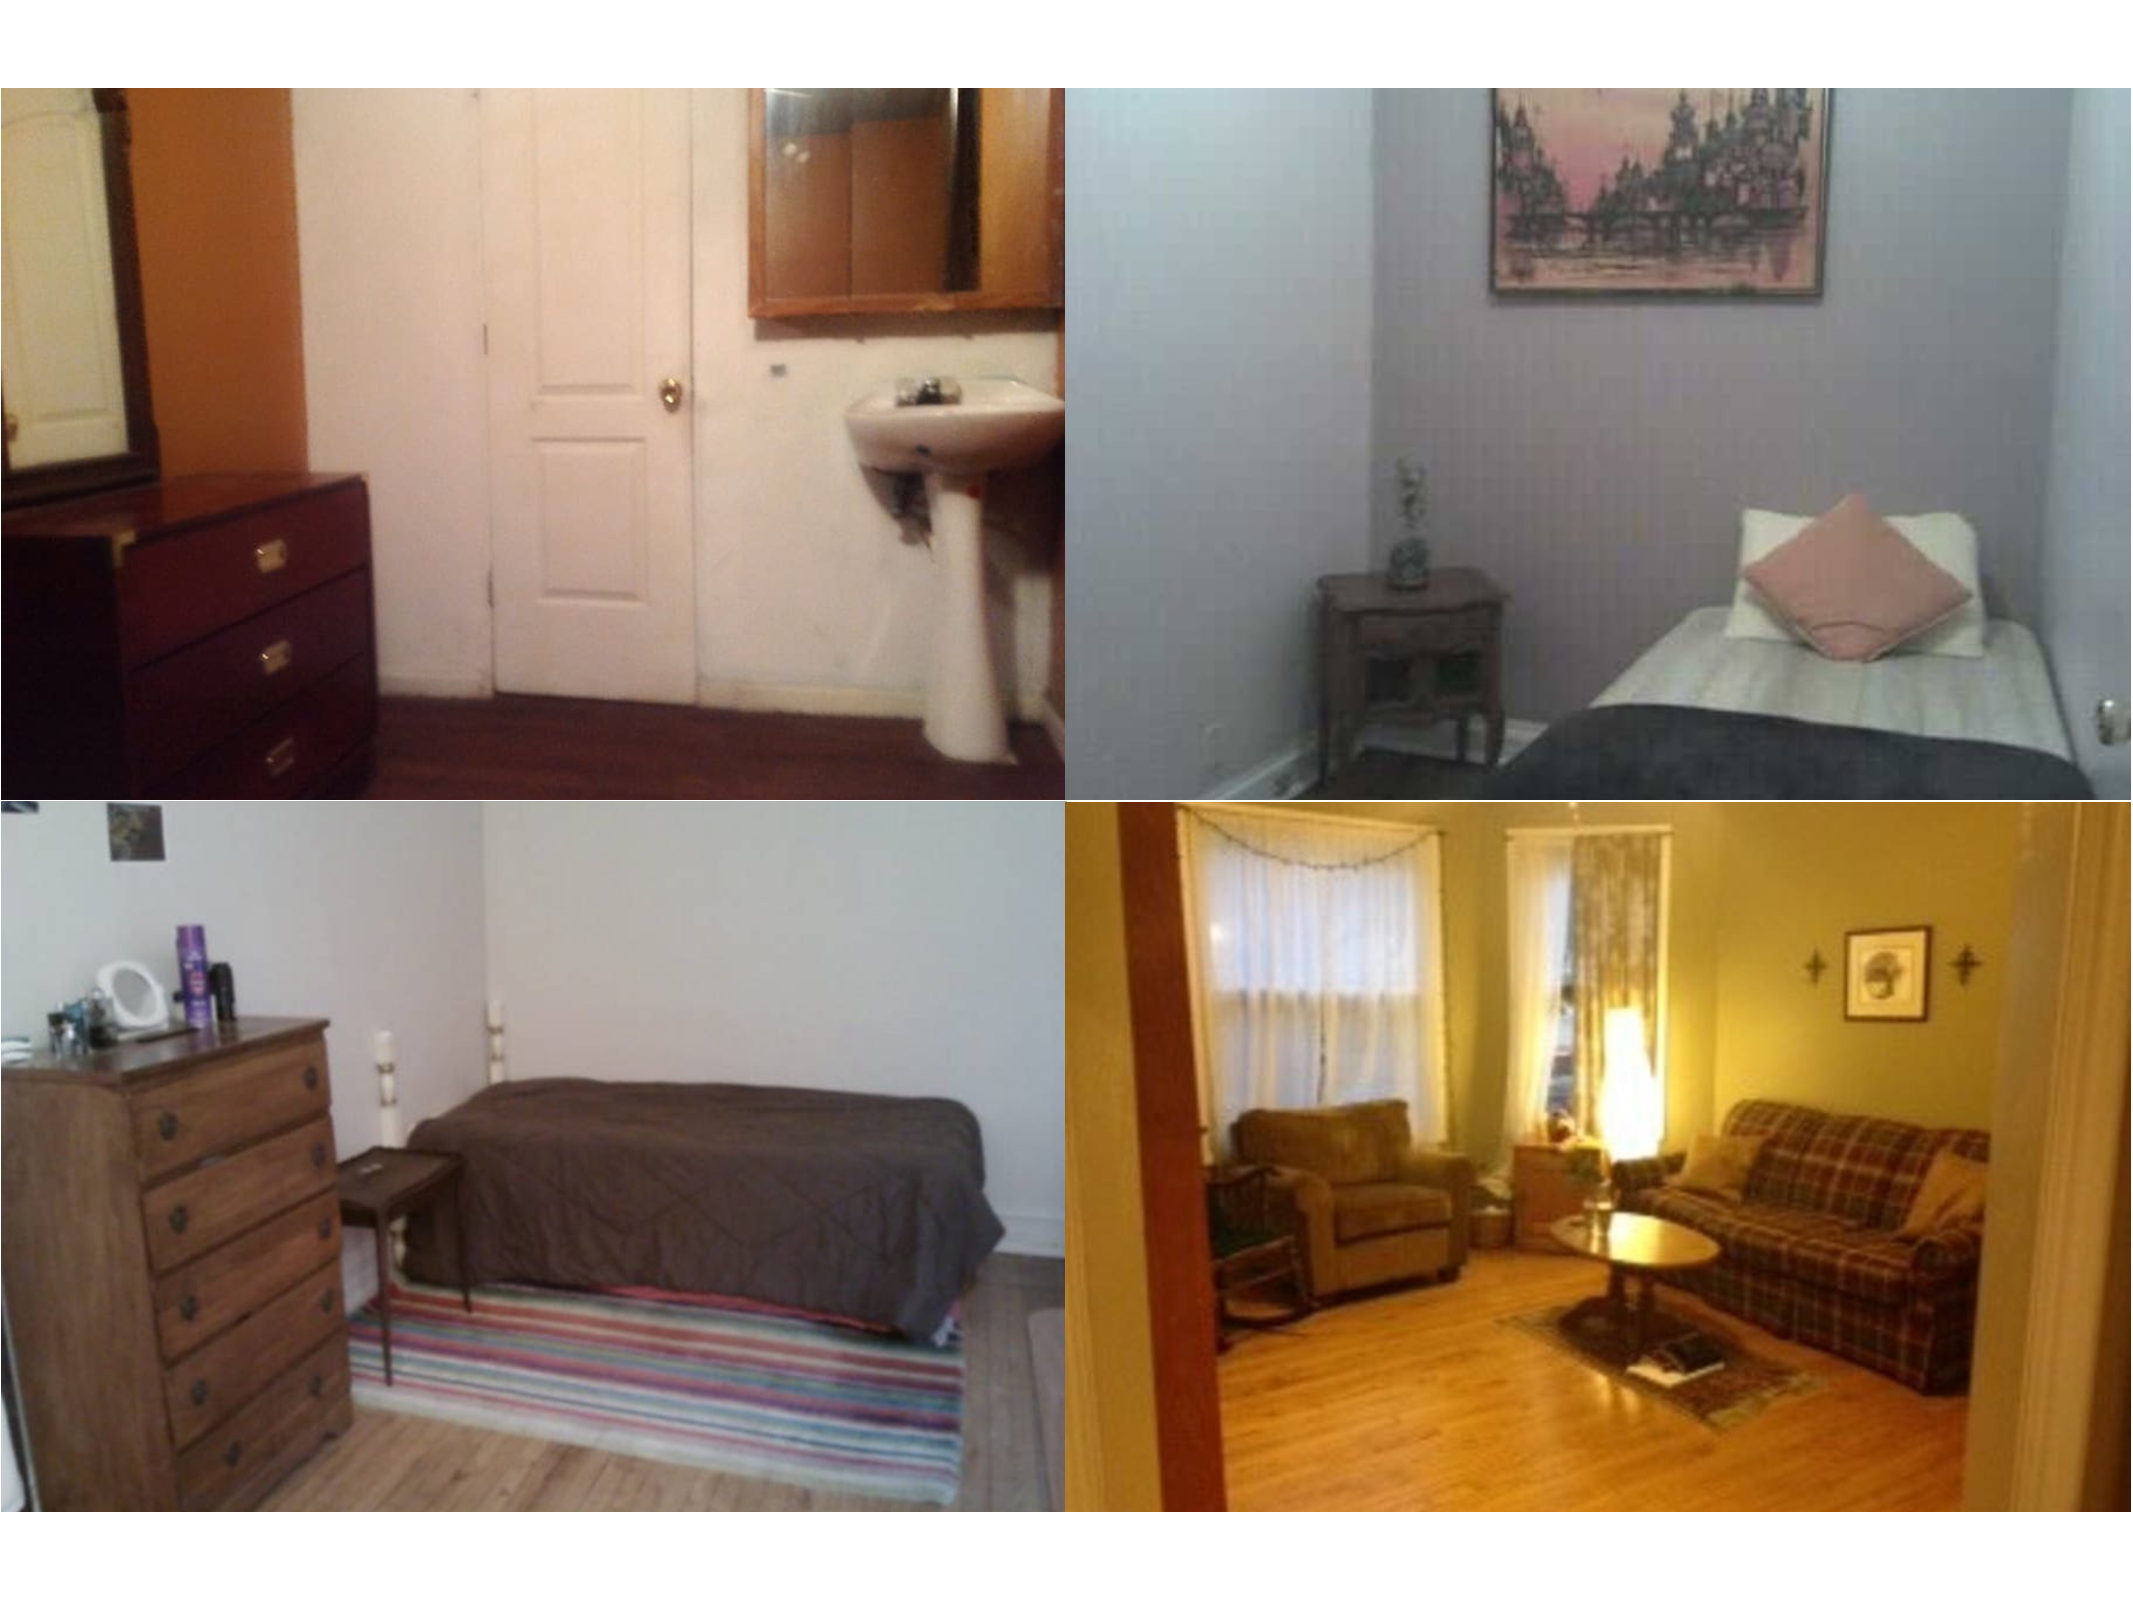
\includegraphics[width=0.4\columnwidth]{pics/low.pdf}
%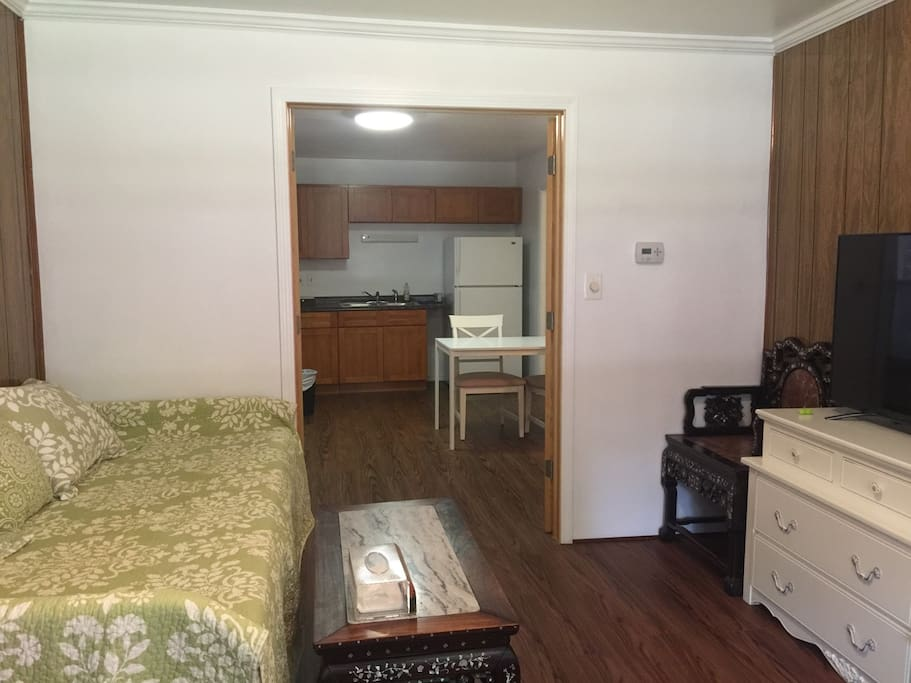
\includegraphics[scale=0.1]{pics/medium/13890897.jpg}
%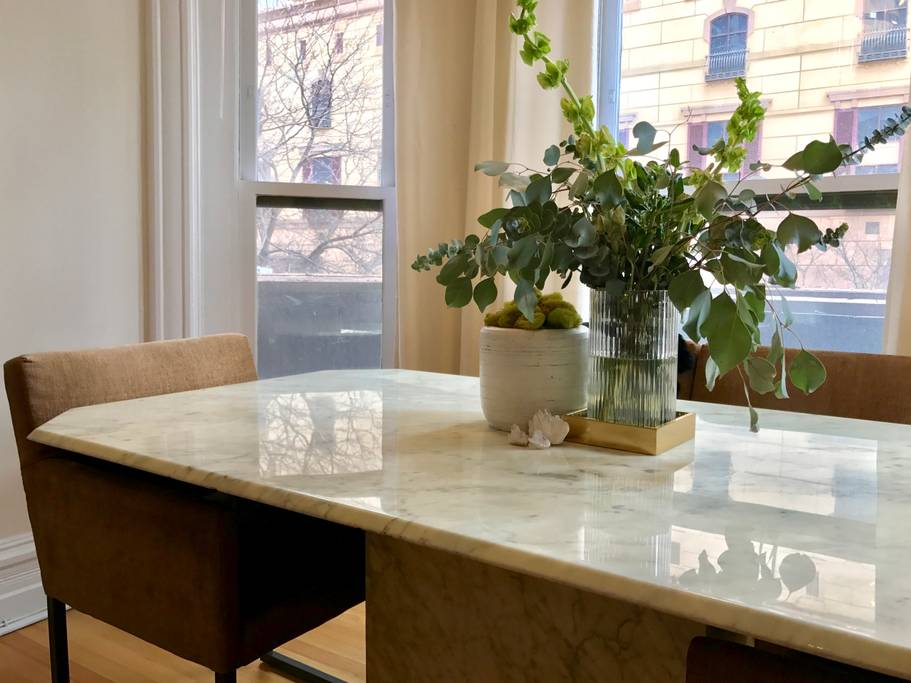
\includegraphics[scale=0.1]{pics/medium/17909111.jpg}
%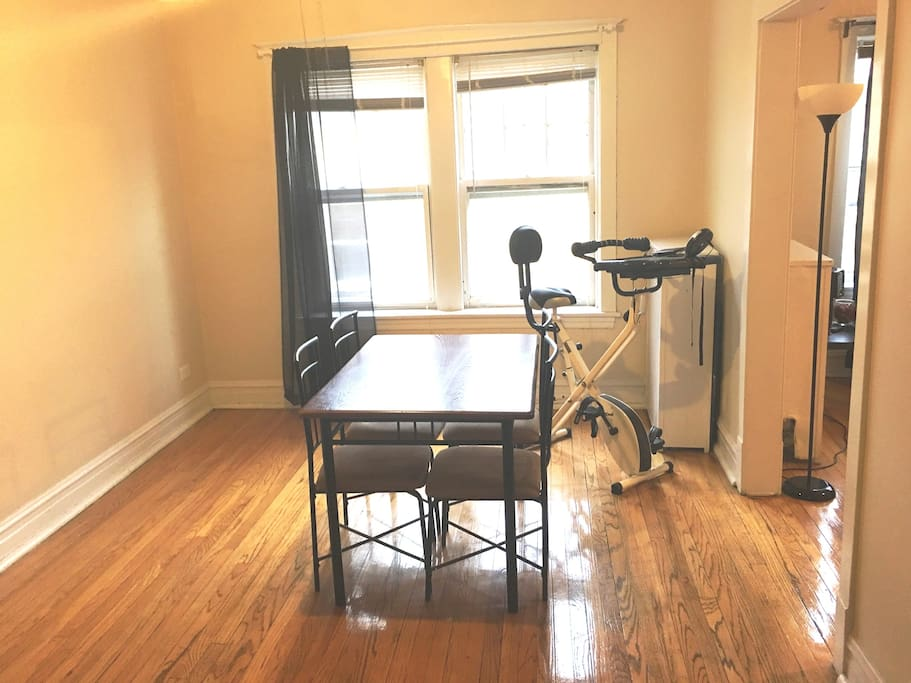
\includegraphics[scale=0.1]{pics/medium/18157129.jpg}
%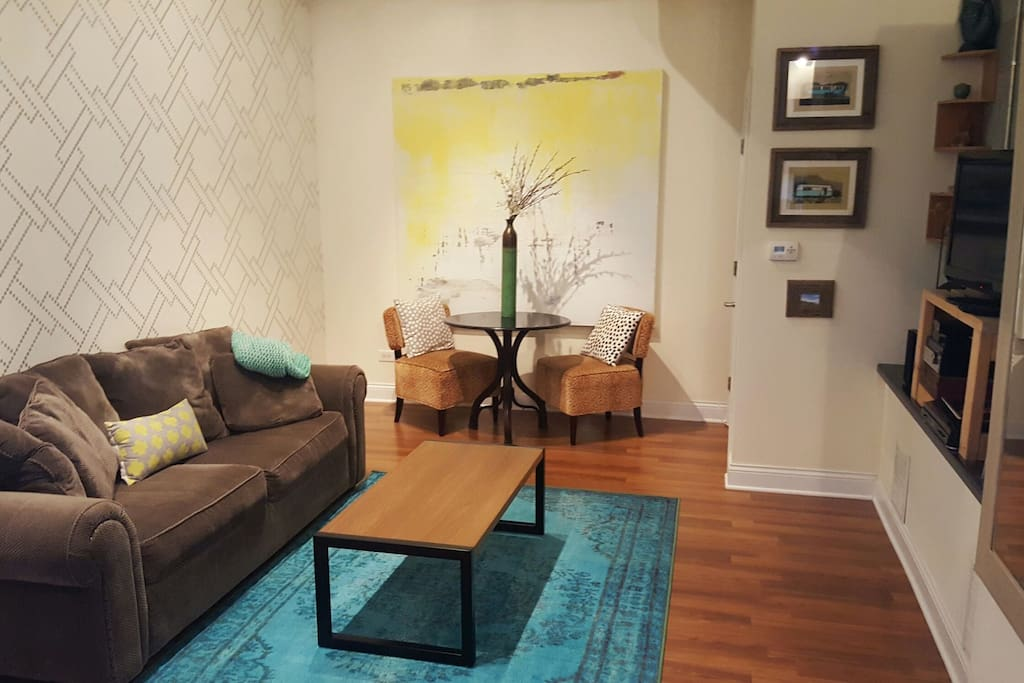
\includegraphics[scale=0.1]{pics/medium/13149571.jpg}
%\\
%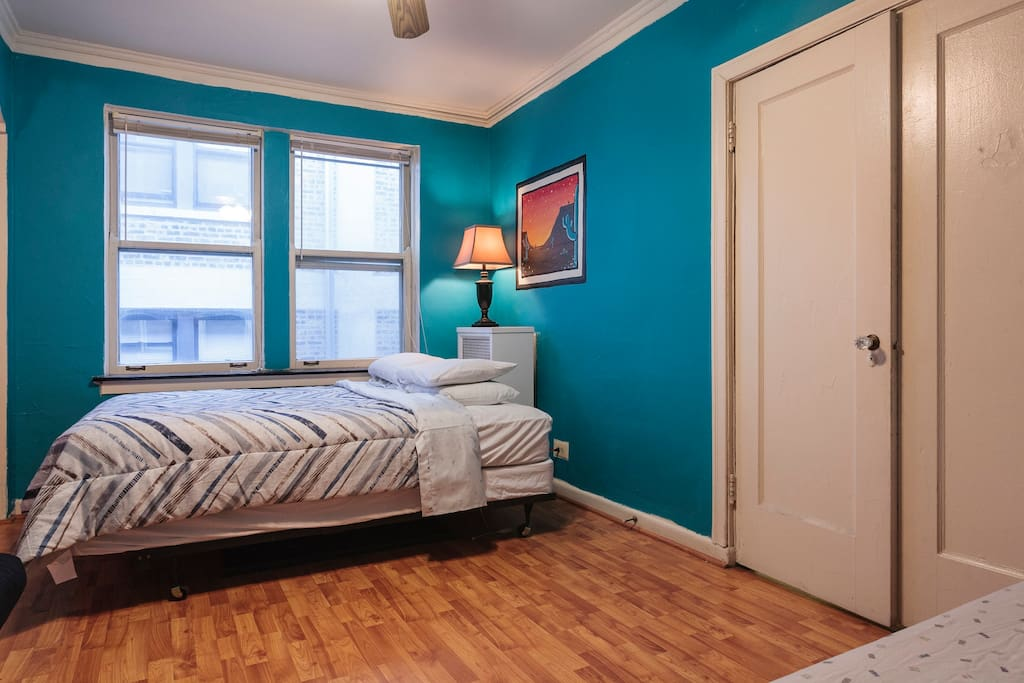
\includegraphics[width=0.5\columnwidth]{pics/high/8207547.jpg}
%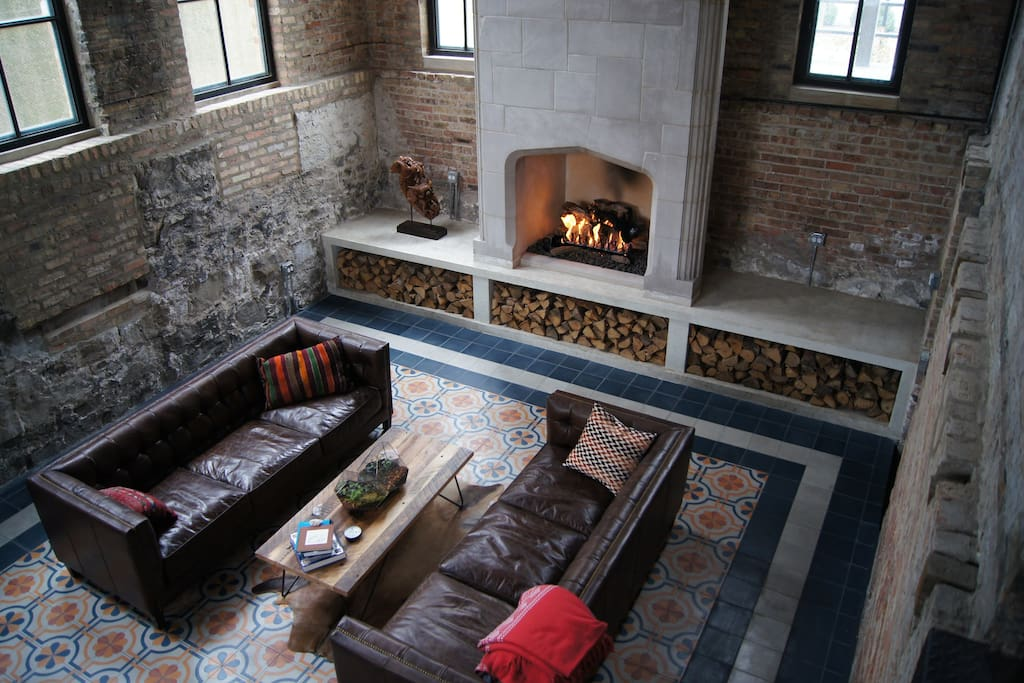
\includegraphics[width=0.5\columnwidth]{pics/high/16812497.jpg}
%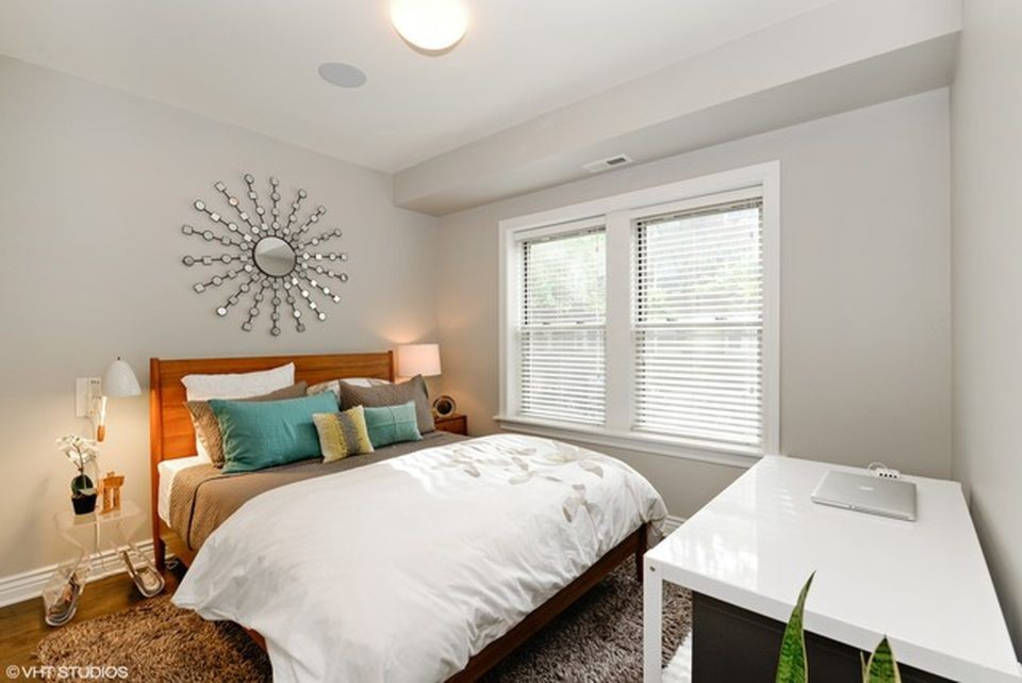
\includegraphics[width=0.5\columnwidth]{pics/high/17253265.jpg}
%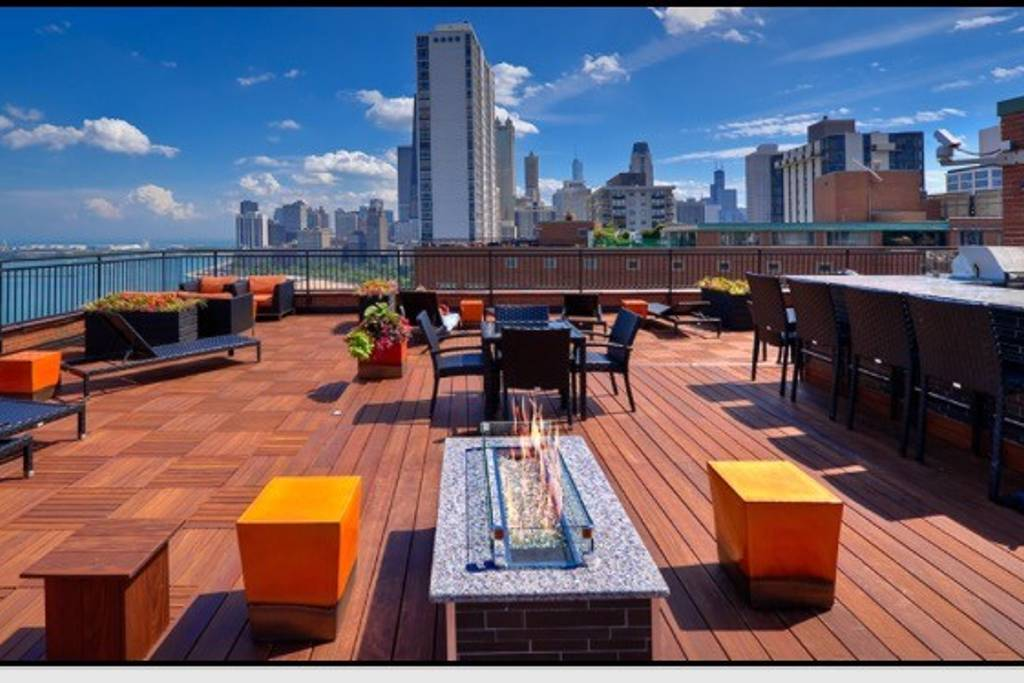
\includegraphics[width=0.5\columnwidth]{pics/high/18061514.jpg}
\includegraphics[width=0.4\columnwidth]{pics/high.pdf}
\caption{Example of images with  low and high  aesthetic score calculated based on ILGNet~\cite{ilgnet}.}
\label{fig:aesimages}
\end{center}
\end{figure*}


\subsection{Airbnb Dataset}
\ab \ does not provide an API to access their dataset, therefore for our study we relied on external sources that collected listings. More specifically we used the listings of Chicago that were last  scraped in May 2017 by InsideAirbnb\footnote{http://insideairbnb.com/ last retrieved on Jan 2018 }; an independent, non-commercial website that provides set of tools and data that allows everyone to explore how Airbnb is really being used in cities around the world.

This dataset includes the all the listed properties in the Chicago region along with the  following  information about the hosts and property. Specifically we consider the following attributes: 

\begin{itemize}
\item Host:  name, photo URL, the date the host joined \ab, the number of listings they have, whether they are a super-host\footnote{Super-hosts in the \ab \ platform are those who hosted at least 10 trips, maintaining at least a 90\%  response rate and received  a 5-star for  at least 80\% of the time they have been reviewed.} or not and finally information on the number of reviews and a user generated scores broken down by communication, interaction and location.

\item{Property}:  photo URL,  price, type of the property (Private/Shared room or Entire Place) as well as  latitude and longitude. 

\end{itemize}

The dataset includes 5200 listings of which 60\% are for renting the entire home/apartment. Moreover, these listings are offered by 3500 uniques hosts. Indeed, the dataset in hand presents that 48\% of the listings are by hosts who offer more than one property, with some of the hosts offering up to one hundred different rooms and houses. These hosts often present lodging business or state agents who use \ab \ platform to rent their various properties.  In this paper as we are interested to uncover social inequality on the individual scale, we filter out all those hosts (and their listings) that have more than one property presented in Chicago during the same time period that the dataset was scrapped. The resulting dataset includes 2700 listings by same number of hosts. 
 
 %final set of features we use
%properties of the dataset 
 
\subsection{American Community Survey}
In addition to the \ab \ dataset we also required information about the socio-economic status of the hosts. We gathered median household income data (Figure~\ref{fig:census}) from the 2016  American Community Survey (ACS). This metric is known as an indicator of socioeconomic status~\cite{li2013spatial}. It is also been shown to be highly correlated with education and unemployment. We also collected the number of household units and the population of \aam, White and Asian households per tract from the ACS (Figure~\ref{fig:census}) .  Throughout our analysis, we chose the level of the census tracts \footnote{Census tracts are geographic areas defined by the U.S. census and generally have a population size between 1,200 and 8,000 people, with an optimum size of 4,000 people.} in terms of granularity as it provides us with a relatively small geographical unit.  Furthermore it allows us to  keep consistent and thus making our findings comparable with other  geographical studies~\cite{Thebault-Spieker17} on the sharing economy.  By combining this dataset with the host demographics identified through photo identification, we calculate an ethnical discrepancy metric for each census tracts as we will describe in the next section. 
 
  
\begin{figure*}[!h]
\begin{center}
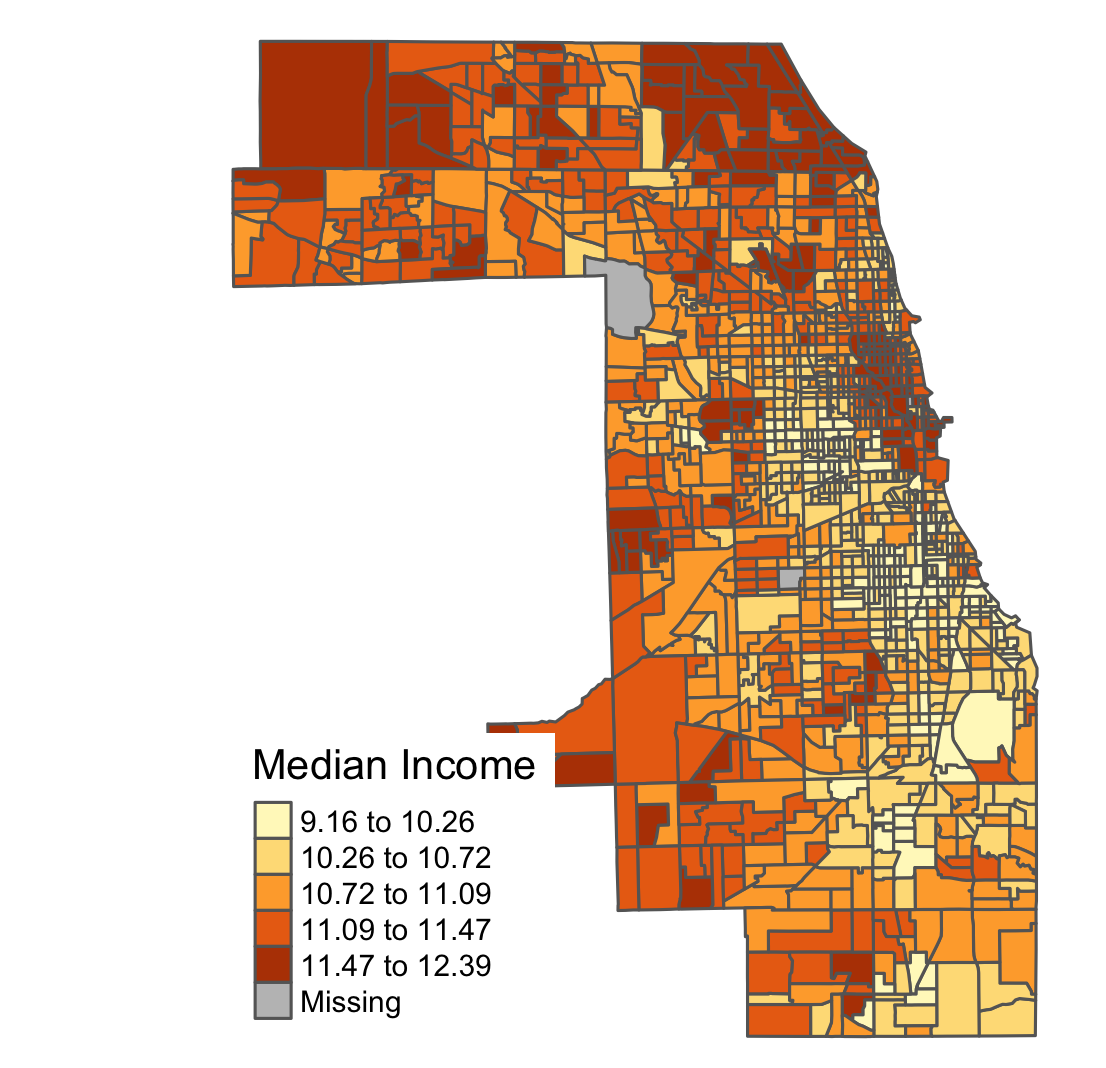
\includegraphics[scale=0.13]{pics/income.png}
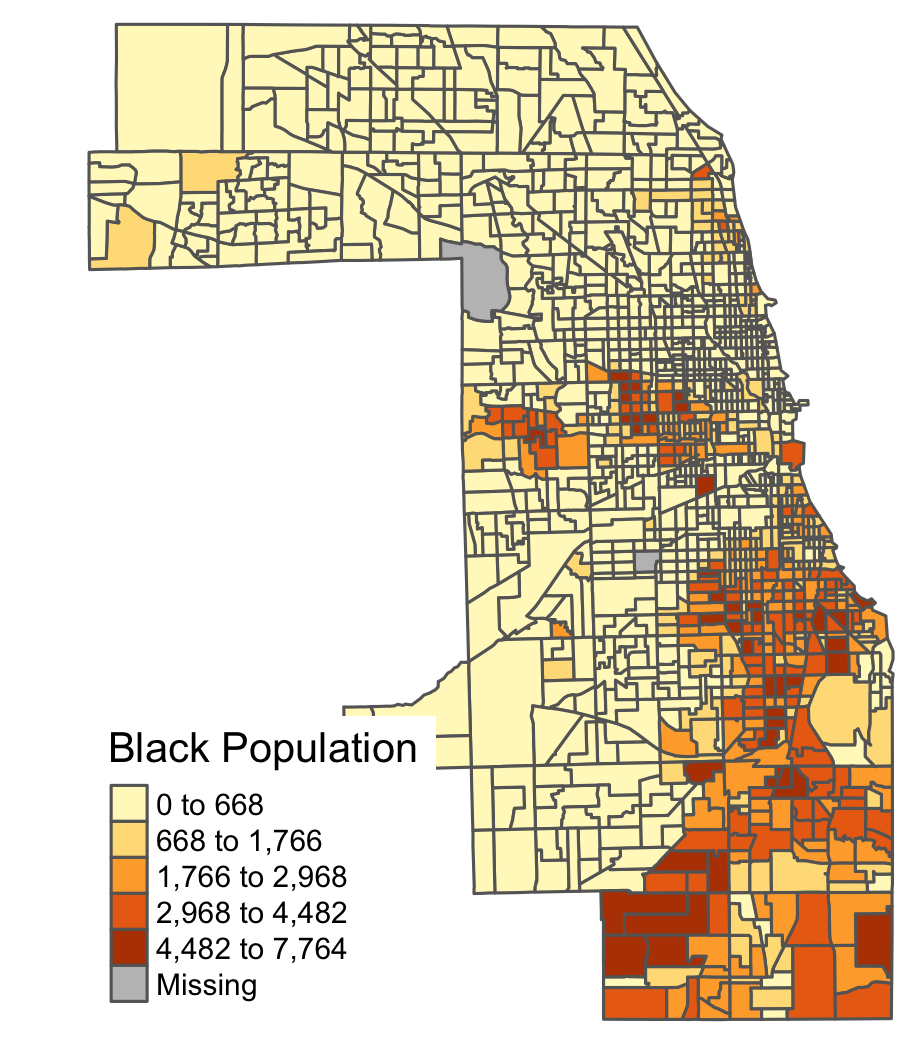
\includegraphics[scale=0.13]{pics/black-census.png}
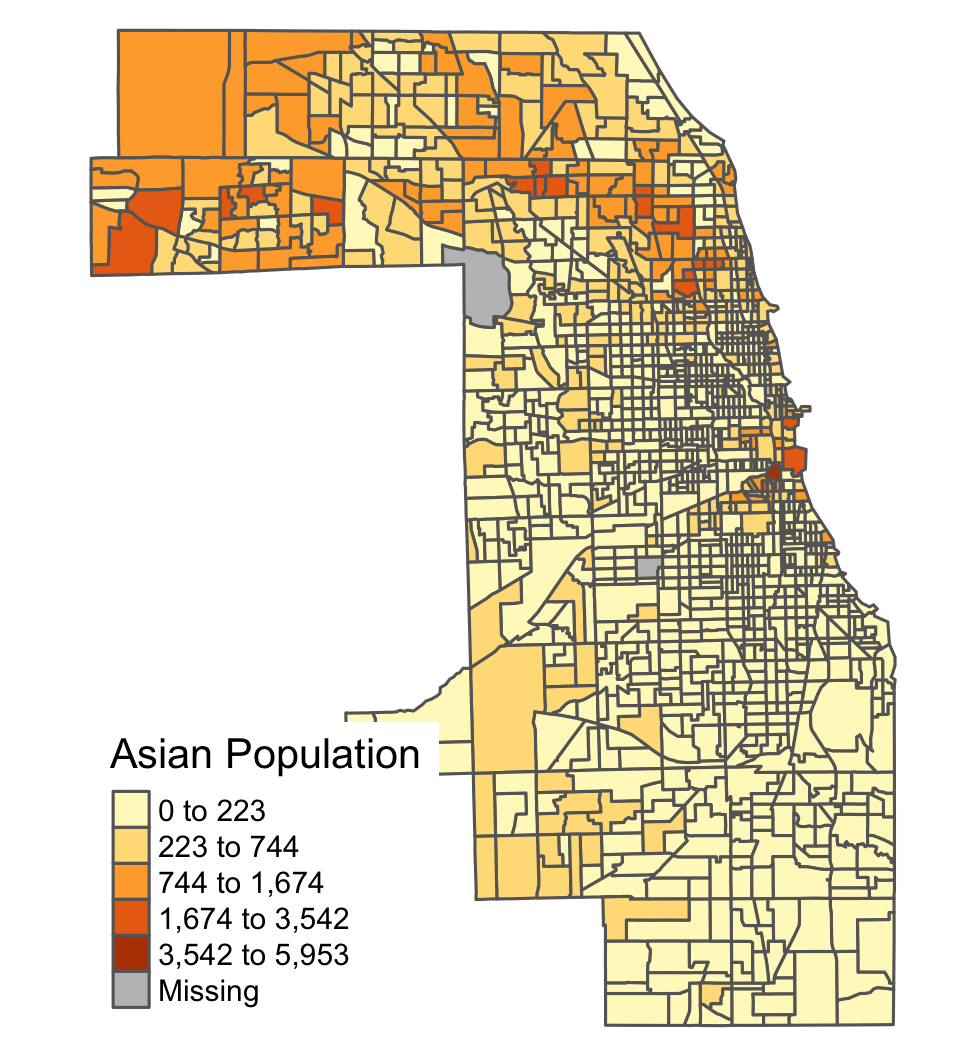
\includegraphics[scale=0.13]{pics/asian-census.png}

\caption{Median household income (in log scale), geographical distribution of \aam \ population, and geographical distribution of Asian population in the greater Chicago area based on the  2016  American Community Survey Data.}
\label{fig:census}
\end{center}
\end{figure*}

\subsection{Demographic Analysis}

\ab \ does not provide any demographic information regarding the host. Therefore we required a technique to automatically detect gender, age and ethnicity. There are currently two possible techniques to do so: one is to process the textual content such as name and the description of the host, to detect the demographics. However this method is known to be error prone as hosts can present themselves with nicknames or arbitrary usernames, and the language used in providing the description of themselves is likely to follow a formal template, making it hard to detect age and the language skill of the writer. An alternative method is to extract demographic data using the host profile picture.  Relying on the latter choice we crawled the host profile photos from the \ab \ website and used the Face++\footnote{Face++. http://en.faceplusplus.com/, 2013.} API to process them. Face++ provides a set of  powerful, and cross-platform vision services which enable us to detect age, gender and race through facial recognition techniques. The API does not provide an estimation of accuracy, however studies that used this API for the similar identification purpose such as~\cite{bakhshi2014faces} have reported of 97\% accuracy when validated against crowd-sourced Mechanical Turk platforms.

\subsection{Aesthetic Analysis}
In order to quantify the aesthetic level of images that hosts present in \ab \ we used advances in deep convolutional neural
network (DCNN) that capture both global and local features.  Local characteristics include noise, blur and contrast while global characteristics include composition features such as rule of thirds, foreground/background separation, depth of field etc. 
In particular we used ILGNet~\cite{ilgnet} a DCNN based algorithm which  introduces the inception module that connects two intermediate local layers to the last layer which extracts the global features for the output. Furthermore this algorithm is based on a pre-trained image classification CNN called GoogLeNet on the ImageNet dataset and  fine tuned on the Aesthetic Visual Analysis (AVA), is a large dataset formed by more than 250 thousands of images~\cite{murray2012ava}. Figure~\ref{fig:aesimages} shows an example of the photos that were classified with a high and low aesthetic score.

